% MeanFlow StormCast -- overall training workflow (trainer_meanflow.py).
% Macro view of one optimization step: data -> frozen regression -> condition
% & residual -> MeanFlow objective -> backward -> AdamW/EMA, with the periodic
% validation branch. Notation: X_{t-1} prev HighRes state, S_t ERA5 background,
% I invariants, M_t = F_xi(...) regression mean, R_t = X_t - M_t residual,
% c_t = concat(X_{t-1}, M_t, I).
\documentclass[border=12pt]{standalone}
% Shared style for the MeanFlow thesis figures.
% Clean academic grayscale, in the spirit of the nntikz examples
% (rounded gray!10 blocks, -latex arrows). Self-contained: this does NOT
% depend on the legacy presentation/meanflow_workflow/src/mf_style.tex.
\usepackage{amsmath,amssymb,bm}
\usepackage{tikz}
\usetikzlibrary{positioning,arrows.meta,calc,fit,backgrounds,shapes.geometric,chains,decorations.pathmorphing}

\tikzset{
  % --- generic nodes ---------------------------------------------------
  base/.style    ={rounded corners=2.5pt, draw, line width=0.8pt, align=center,
                   inner sep=5pt, font=\small, text=black!88},
  block/.style   ={base, fill=gray!10},
  data/.style    ={base, fill=white},                       % data / tensors
  net/.style     ={base, fill=gray!22, line width=1.0pt},   % trained network
  frozen/.style  ={base, fill=gray!4, draw=black!60,        % frozen network
                   dash pattern=on 3pt off 2pt},
  loss/.style    ={base, fill=gray!10, line width=1.0pt,    % loss / scalar
                   double, double distance=1.2pt},
  emph/.style    ={base, fill=gray!10, line width=1.3pt},   % highlighted box
  % --- operator glyphs -------------------------------------------------
  op/.style      ={circle, draw, line width=0.8pt, fill=white,
                   minimum size=4.6mm, inner sep=0, font=\footnotesize},
  concat/.style  ={rectangle, rounded corners=1pt, draw, fill=black!72,
                   text=white, font=\scriptsize\bfseries, inner sep=2.5pt},
  % --- arrows ----------------------------------------------------------
  arrow/.style   ={-{Latex[length=2.4mm]}, line width=0.8pt, draw=black!82},
  arrowc/.style  ={arrow, rounded corners=3pt},
  thinarrow/.style={-{Latex[length=2.0mm]}, line width=0.6pt, draw=black!55},
  loopback/.style={-{Latex[length=2.4mm]}, line width=0.8pt, draw=black!55,
                   dashed, dash pattern=on 4pt off 3pt},
  % --- containers / annotation ----------------------------------------
  group/.style   ={rounded corners=5pt, draw=black!40, line width=0.7pt,
                   dashed, dash pattern=on 3pt off 2.5pt, fill=black!2,
                   inner sep=8pt},
  ttl/.style     ={font=\bfseries\large, text=black!88},
  sub/.style     ={font=\itshape\footnotesize, text=black!55},
  lab/.style     ={font=\scriptsize, text=black!70},
  tag/.style     ={font=\scriptsize\bfseries, text=black!60},
  % small sine glyph used to mark Fourier / positional embeddings
  sinewave/.style={decorate, decoration={snake, amplitude=0.6mm,
                   segment length=2.2mm}},
}

% legend swatch helper: \swatch{<style>}{<label>}
\newcommand{\swatch}[2]{%
  \tikz[baseline=-0.5ex]\node[#1, minimum width=3.6mm, minimum height=2.8mm,
    inner sep=0]{};\;#2}

\begin{document}
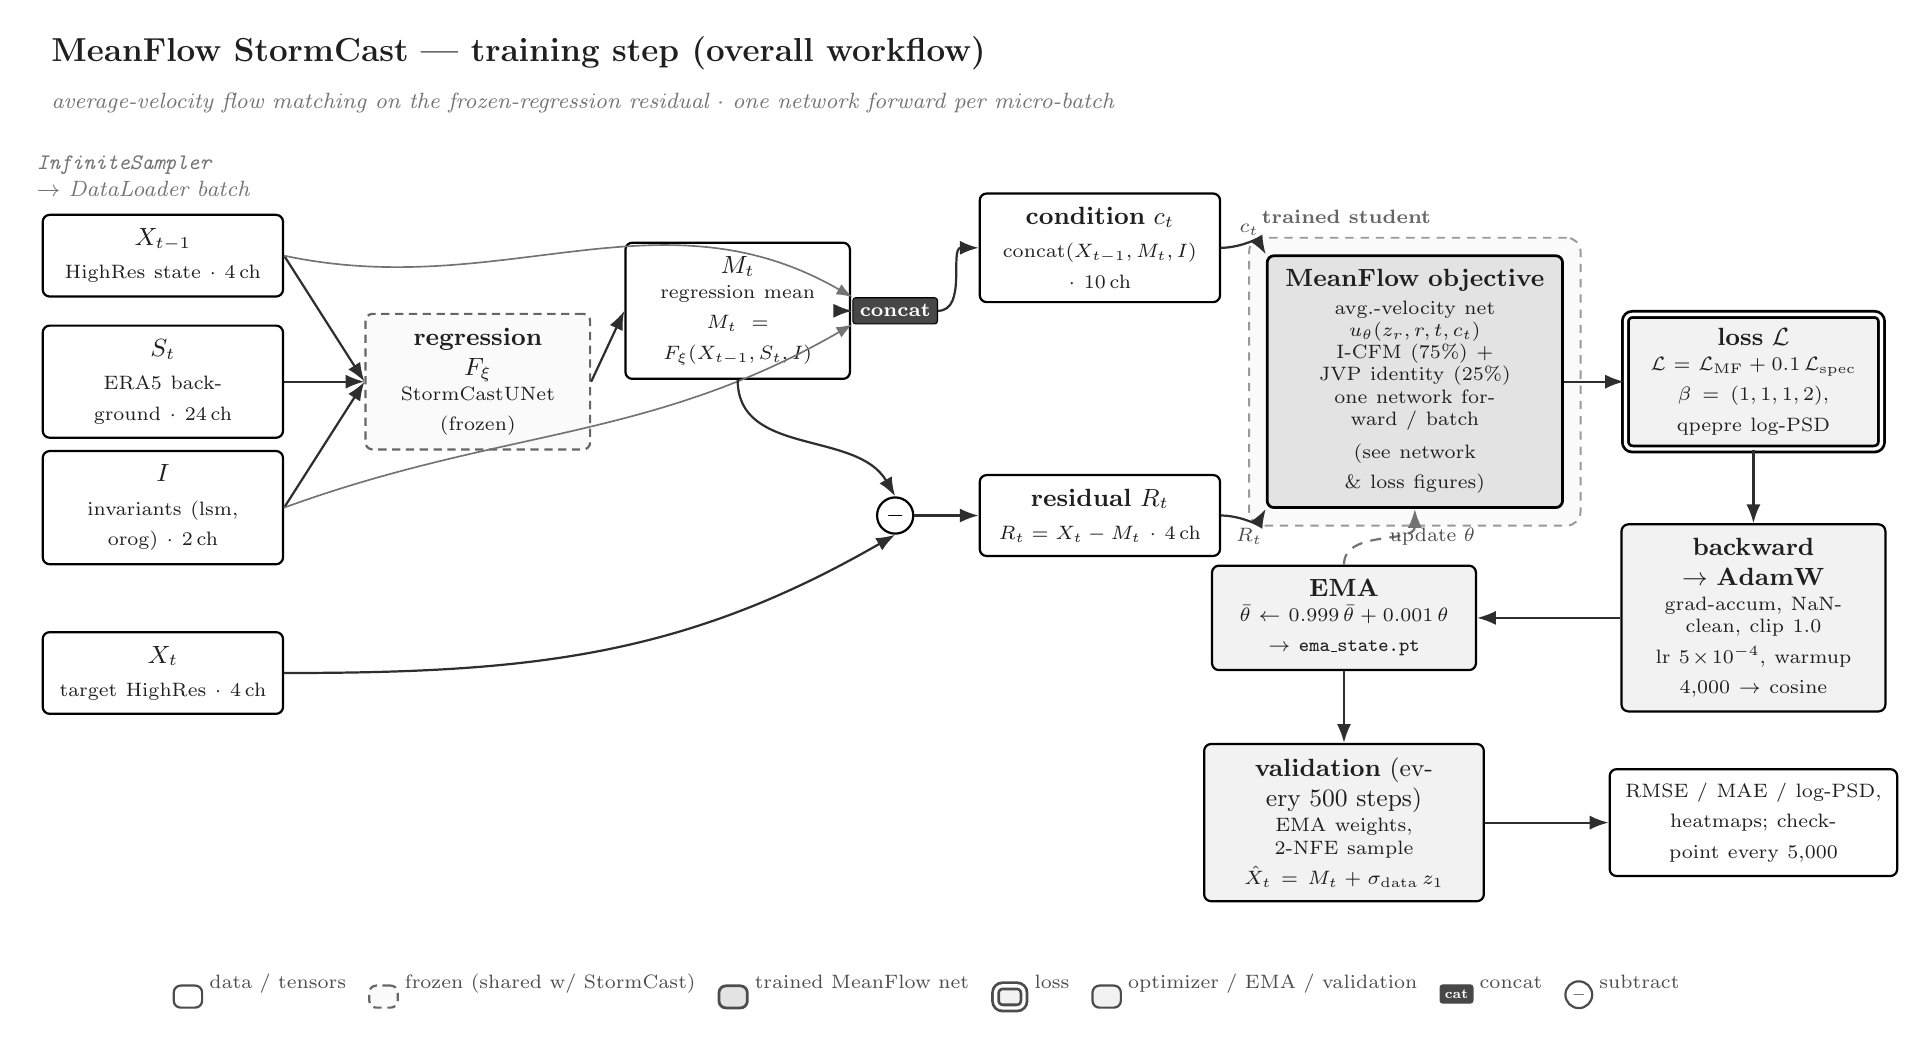
\begin{tikzpicture}[node distance=9mm]

  % ============================= inputs (a batch) =============================
  \node[data, text width=2.7cm] (xprev) at (0,1.6)  {$X_{t-1}$\\[1pt]\scriptsize HighRes state $\cdot$ 4\,ch};
  \node[data, text width=2.7cm] (st)    at (0,0)     {$S_t$\\[1pt]\scriptsize ERA5 background $\cdot$ 24\,ch};
  \node[data, text width=2.7cm] (inv)   at (0,-1.6)  {$I$\\[1pt]\scriptsize invariants (lsm, orog) $\cdot$ 2\,ch};
  \node[data, text width=2.7cm] (xt)    at (0,-3.7)  {$X_t$\\[1pt]\scriptsize target HighRes $\cdot$ 4\,ch};

  \node[sub, anchor=south, text width=3.2cm] at ($(xprev.north)+(0,1mm)$)
    {\texttt{InfiniteSampler}\\$\to$ DataLoader batch};

  % ===================== Phase 1: frozen regression =====================
  \node[frozen, text width=2.5cm] (reg) at (4.0,0)
    {\textbf{regression}\\$F_\xi$\\[1pt]\scriptsize StormCastUNet\\(frozen)};
  \node[data, text width=2.5cm] (mt) at (7.3,0.9)
    {$M_t$\\[1pt]\scriptsize regression mean\\$M_t=F_\xi(X_{t-1},S_t,I)$};

  % ----- conditioning bundle (concat) and residual target (subtract) -----
  \node[concat] (cc)  at (9.3,0.9) {concat};
  \node[data, text width=2.7cm] (cond) at (11.9,1.7)
    {\textbf{condition} $c_t$\\[1pt]\scriptsize $\mathrm{concat}(X_{t-1},M_t,I)$ $\cdot$ 10\,ch};
  \node[op] (sub) at (9.3,-1.7) {$-$};
  \node[data, text width=2.7cm] (resid) at (11.9,-1.7)
    {\textbf{residual} $R_t$\\[1pt]\scriptsize $R_t=X_t-M_t$ $\cdot$ 4\,ch};

  % ===================== Phase 2: MeanFlow objective (highlighted) =====================
  \node[net, text width=3.4cm] (mf) at (15.9,0)
    {\textbf{MeanFlow objective}\\[2pt]\scriptsize avg.-velocity net $u_\theta(z_r,r,t,c_t)$\\
     I-CFM (75\%) $+$ JVP identity (25\%)\\one network forward / batch\\[1pt](see network \& loss figures)};
  \begin{scope}[on background layer]
    \node[group, fit=(mf), inner sep=6pt] (p2) {};
  \end{scope}
  \node[tag, anchor=south west] at ($(p2.north west)+(0.5mm,0.4mm)$) {trained student};

  % ----- loss scalar -----
  \node[loss, text width=2.9cm] (loss) at (20.2,0)
    {\textbf{loss} $\mathcal L$\\[1pt]\scriptsize $\mathcal L=\mathcal L_{\mathrm{MF}}+0.1\,\mathcal L_{\mathrm{spec}}$\\
     $\beta=(1,1,1,2)$, qpepre log-PSD};

  % ===================== backward + optimizer + EMA =====================
  \node[block, text width=3.0cm] (opt) at (20.2,-3.0)
    {\textbf{backward $\to$ AdamW}\\[1pt]\scriptsize grad-accum, NaN-clean, clip $1.0$\\
     lr $5\!\times\!10^{-4}$, warmup $4{,}000$ $\to$ cosine};
  \node[block, text width=3.0cm] (ema) at (15.0,-3.0)
    {\textbf{EMA}\\[1pt]\scriptsize $\bar\theta\leftarrow0.999\,\bar\theta+0.001\,\theta$\\
     $\to$ \texttt{ema\_state.pt}};

  % ===================== periodic validation branch =====================
  \node[block, text width=3.2cm] (val) at (15.0,-5.6)
    {\textbf{validation} (every 500 steps)\\[1pt]\scriptsize EMA weights, 2-NFE sample\\
     $\hat X_t=M_t+\sigma_{\mathrm{data}}\,z_1$};
  \node[data, text width=3.3cm] (metrics) at (20.2,-5.6)
    {\scriptsize RMSE / MAE / log-PSD,\\heatmaps; checkpoint every 5{,}000};

  % ============================= edges =============================
  % phase 1: inputs -> regression
  \draw[arrow] (xprev.east) -- (reg.west);
  \draw[arrow] (st.east)    -- (reg.west);
  \draw[arrow] (inv.east)   -- (reg.west);
  \draw[arrow] (reg.east)   -- (mt.west);
  % condition (concat): X_{t-1}, M_t, I -> cc -> cond
  \draw[arrow]     (mt.east)   -- (cc.west);
  \draw[thinarrow] (xprev.east) to[out=-12,in=150] (cc.north west);
  \draw[thinarrow] (inv.east)  to[out=20,in=210] (cc.south west);
  \draw[arrow] (cc.east) to[out=0,in=180] (cond.west);
  % residual (subtract): M_t - X_t -> resid
  \draw[arrow] (mt.south)  to[out=-90,in=120] (sub.north);
  \draw[arrow] (xt.east)   to[out=0,in=210] (sub.south);
  \draw[arrow] (sub.east)  -- (resid.west);
  % into MeanFlow objective
  \draw[arrow] (cond.east)  to[out=0,in=120] node[lab,above,pos=0.55]{$c_t$} (mf.north west);
  \draw[arrow] (resid.east) to[out=0,in=240] node[lab,below,pos=0.55]{$R_t$} (mf.south west);
  % objective -> loss -> backward -> ema -> (loop back) student
  \draw[arrow] (mf.east) -- (loss.west);
  \draw[arrow] (loss.south) -- (opt.north);
  \draw[arrow] (opt.west) -- (ema.east);
  \draw[loopback] (ema.north) to[out=90,in=-90] node[lab,right,pos=0.5]{update $\theta$} (mf.south);
  % validation branch
  \draw[arrow] (ema.south) -- (val.north);
  \draw[arrow] (val.east) -- (metrics.west);

  % ============================= title =============================
  \node[ttl, anchor=south west] (title) at ($(xprev.north west)+(0,17mm)$)
    {MeanFlow StormCast --- training step (overall workflow)};
  \node[sub, anchor=north west] at ($(title.south west)+(0,-0.5mm)$)
    {average-velocity flow matching on the frozen-regression residual $\cdot$ one network forward per micro-batch};

  % ============================= legend =============================
  \node[lab, anchor=north west] at (0,-7.4)
    {\swatch{data}{data / tensors}\quad
     \swatch{frozen}{frozen (shared w/ StormCast)}\quad
     \swatch{net}{trained MeanFlow net}\quad
     \swatch{loss}{loss}\quad
     \swatch{block}{optimizer / EMA / validation}\quad
     \tikz[baseline=-0.5ex]\node[concat, scale=0.7]{cat};\;concat\quad
     \tikz[baseline=-0.5ex]\node[op, minimum size=3.4mm]{\tiny$-$};\;subtract};

\end{tikzpicture}
\end{document}
